\section[Kontrast]{Kontrast} % (fold)
\label{sec:kontrastierung}


\subsection{Kontrastentstehung} % (fold)
\label{sub:kontrastentstehung}

\begin{frame}
	\frametitle{Kontrastentstehung}
	\begin{block}{Amplitudenkontrast}
		\begin{itemize}
			\item Elastische Streuung der Elektronen
			\item Stark gestreute Elektronen werden nicht detektiert
			\item Kontrast im Realraum
		\end{itemize}		
	\end{block}
\end{frame}

\begin{frame}
	\frametitle{Kontrastentstehung}
	\begin{block}{Phasenkontrast}
		\begin{itemize}
			\item Elastisch und inelastische Streuung der Elektronen
			\item Phasenverschiebung der Elektronenwellen
			\item Kontrast im Fourierraum
		\end{itemize}
	\end{block}
\end{frame}

\begin{frame}
	\frametitle{Kontrastentstehung}
	\begin{block}{Kontrast-Transfer-Funktion}
		\begin{itemize}
			\item Verbindung zwischen Amplitudenkontrast und Phase
		\end{itemize}
	\end{block}
	\begin{equation*}
		\text{KTF}(\vec{k})=\sqrt{1-A^2}\cdot \sin{(\gamma(\vec{k}))} + A \cdot \cos{(\gamma(\vec{k}))}
	\end{equation*}
	\begin{equation*}
		\gamma(\vec{k}) = -\frac{\pi}{2}C_s \lambda^3 |\vec{k}|^4 + \pi \lambda z(\theta) |\vec{k}|^2
	\end{equation*}
	\begin{figure}
		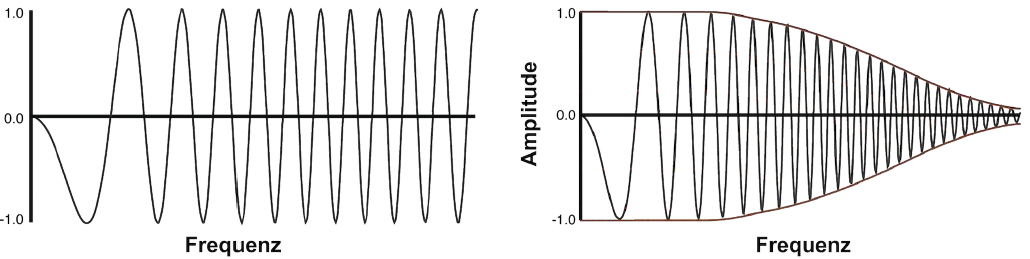
\includegraphics[width = 10cm]{pic/KTF.png}
	\end{figure}
\end{frame}

\subsection{Kontrastierungsmethoden} % (fold)
\label{sub:subsection_name}

\begin{frame}
	\frametitle{Kontrastierungsmethoden}
	\begin{block}{Negativkontrastierung}
		\begin{itemize}
			\item Schwermetalllösung
			\item Hoher Kontrast			
			\item Deformation der Probe
		\end{itemize}
	\end{block}
	\begin{figure}
		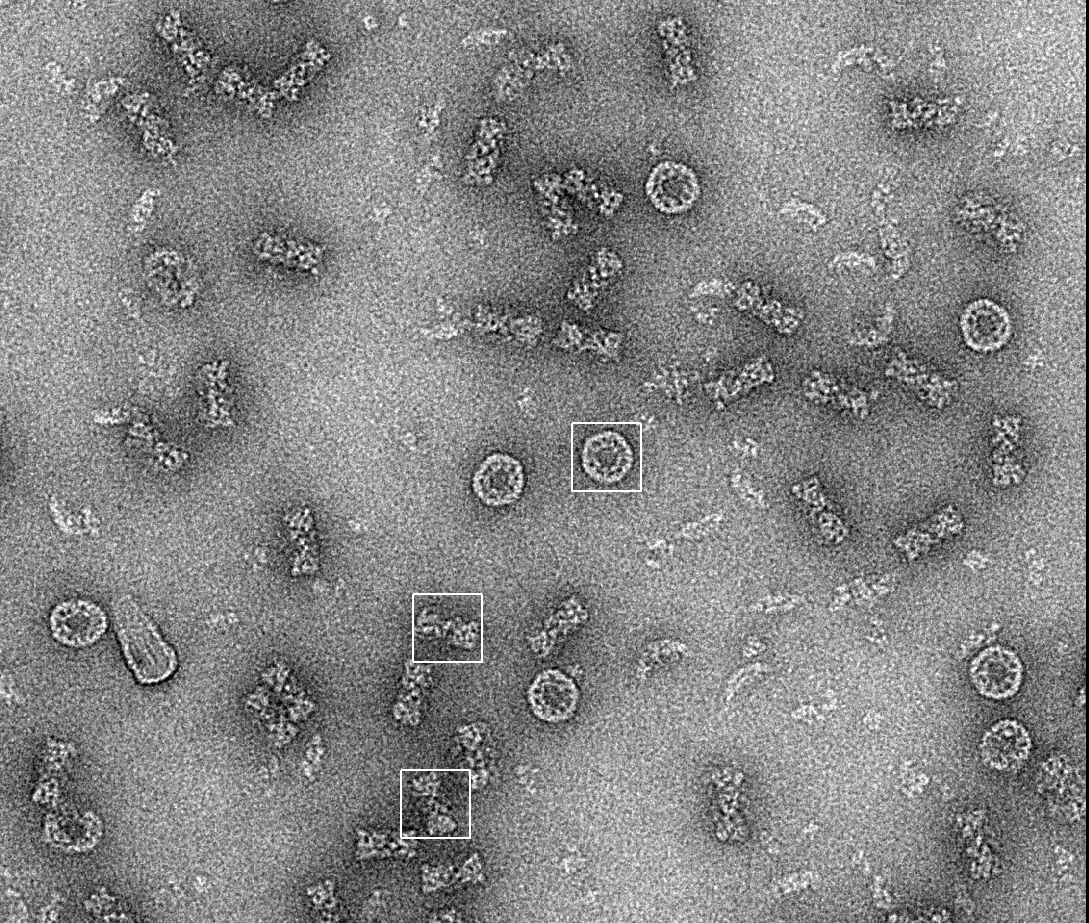
\includegraphics[width = 6cm]{pic/stain.png}
	\end{figure}
\end{frame}
\begin{frame}
	\frametitle{Kontrastierungsmethoden}
	\begin{block}{Kryo-Fixierung}
		\begin{itemize}
			\item Wasserlösung
			\item Geringer Kontrast
			\item Erhalt der Konformation
		\end{itemize}
	\end{block}
	\centering
	\begin{minipage}{5cm}
		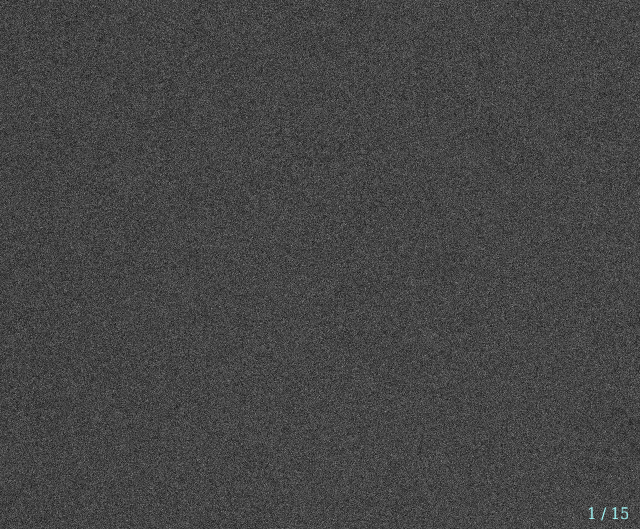
\includegraphics[width = 5cm]{pic/kryo2.png}
	\end{minipage}
	\begin{minipage}{5cm}
		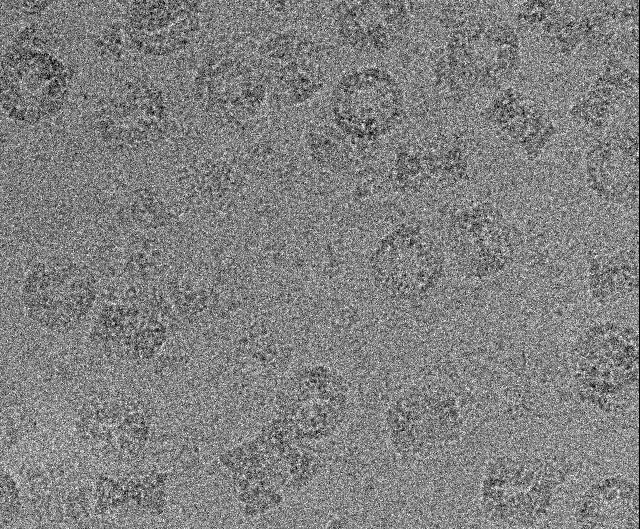
\includegraphics[width = 5cm]{pic/kryo1.png}
	\end{minipage}
\end{frame}
\begin{frame}
	\frametitle{Kontrastierungsmethoden}
	\begin{block}{Cryo-Negativkontrastierung}
		\begin{itemize}
			\item Schwermetalllösung
			\item Vitrifizierung
			\item Beobachtung kleiner Komplexe
			\item Keine normale Umgebung der Probe
		\end{itemize}
	\end{block}
	\begin{figure}
		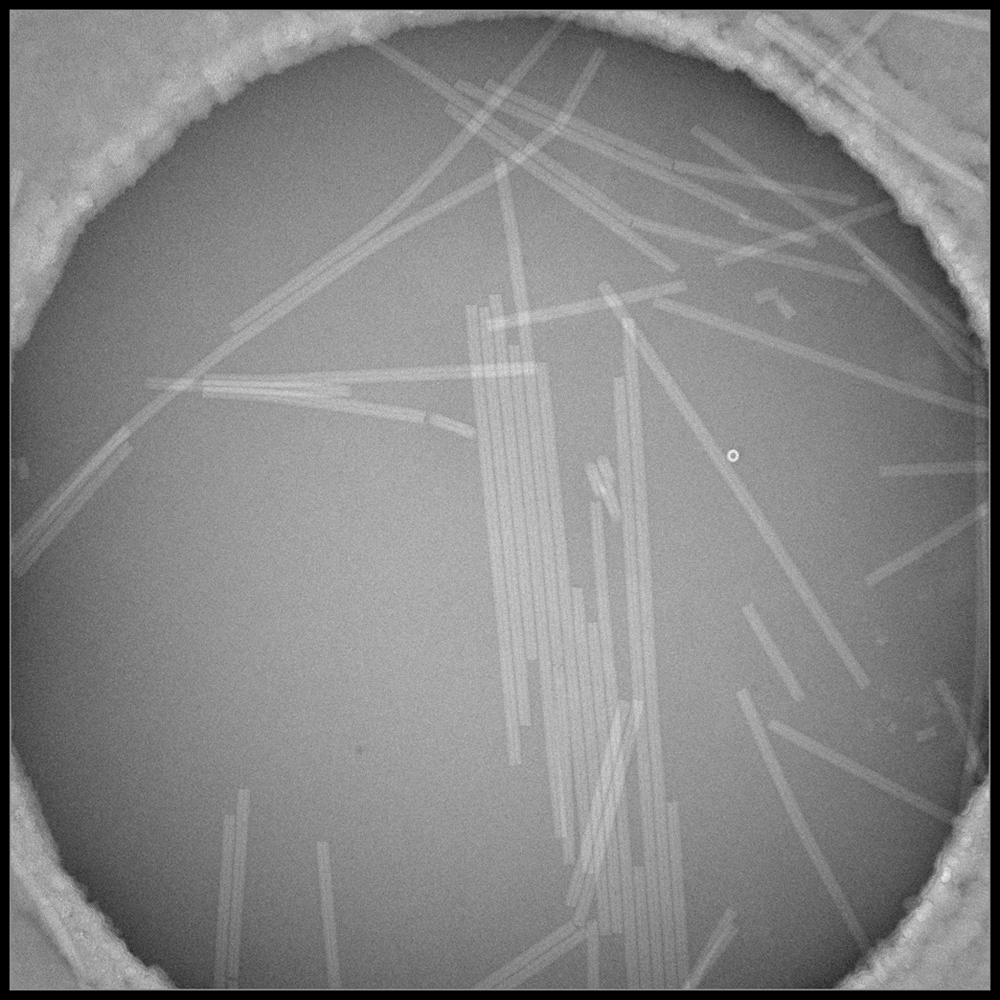
\includegraphics[height = 4cm]{pic/cryostain.png}
	\end{figure}
\end{frame}